





stone\_test: bunch of small tests to make sure all works as expected 

stone.py: computes B on plane or line above 3D domain with mesh

two surface integral functions, one for cuboids, one for deformed hexahedra accomodating surface

jit much faster!









\begin{center}
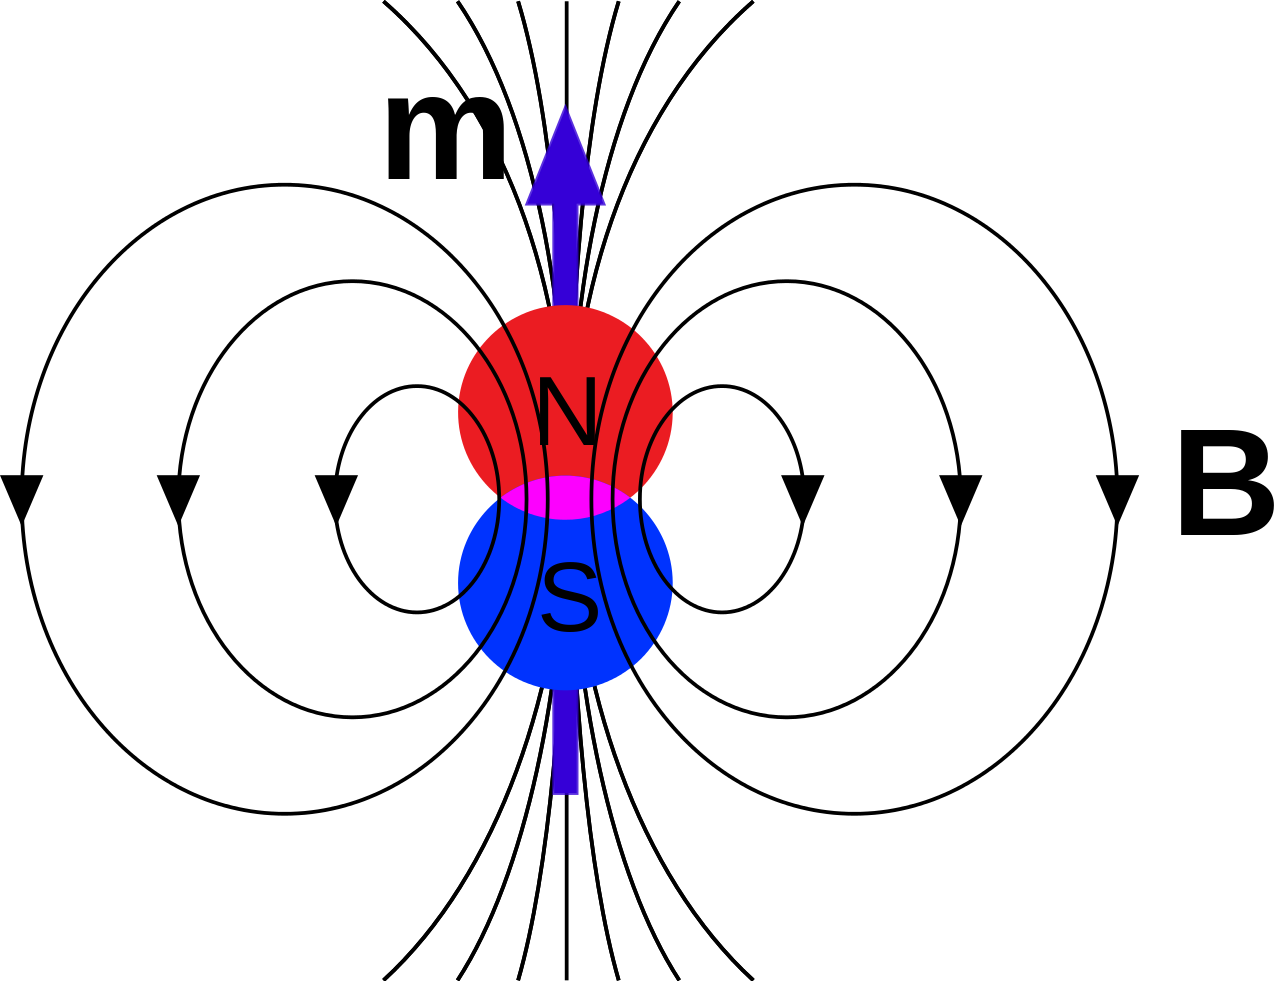
\includegraphics[width=6cm]{python_codes/fieldstone_138/images/Magnetic_field_due_to_dipole_moment.png}
\end{center}

Outside of the source region, this potential is the vector potential $\vec A$ of a magnetic dipole is (
$\vec r$ is the vector from the position of the dipole to the position where the field is being measured):
\[
\vec A(\vec r) = \frac{\mu_0}{4 \pi} \frac{\vec m \times \vec r}{r^3}
\]
and the magnetic flux density field $\vec B$ (in Tesla) is a vector quantity given by
\[
\vec B (\vec r) = \vec \nabla \times \vec A 
=
\frac{\mu_0}{4\pi} \left[  \frac{3 \vec r (\vec m \cdot \vec r)}{r^5} - \frac{\vec m}{r^3}  \right]
\]
Note that a slightly different equation is presented on Wikipedia, which adds a term to the above one:
\[
\vec B (\vec r) = \vec \nabla \times \vec A 
=
\frac{\mu_0}{4\pi} \left[  \frac{3 \vec r (\vec m \cdot \vec r)}{r^5} - \frac{\vec m}{r^3}  \right]
+ \frac{2\mu_0}{3} \vec m \; \delta(\bm r)
\]

From Wiki\footnote{\url{https://en.wikipedia.org/wiki/Magnetization}}: In classical electromagnetism, magnetization or magnetic polarization is the vector field that expresses the density of permanent or induced magnetic dipole moments in a magnetic material. The origin of the magnetic moments responsible for magnetization can be either microscopic electric currents resulting from the motion of electrons in atoms, or the spin of the electrons or the nuclei. Net magnetization results from the response of a material to an external magnetic field, together with any unbalanced magnetic dipole moments that may be inherent in the material itself; for example, in ferromagnets. Magnetization is not always uniform within a body, but rather varies between different points. 
Physicists and engineers usually define magnetization as the quantity of magnetic moment per unit volume. It is represented by a pseudovector $\vec M$.

The magnetization field ($\vec M$-field) can be defined according to the following equation: 
\[
\vec M = \frac{\delta \vec m}{\delta V}
\]
Where $\delta \vec m$ is the elementary magnetic moment and $\delta V$  
is the volume element; in other words, the $\vec M$-field 
is the distribution of magnetic moments in the region or manifold concerned. 
This is better illustrated through the following relation:
\[
\vec m = \int\int\int \vec M \; dV
\]

\begin{center}
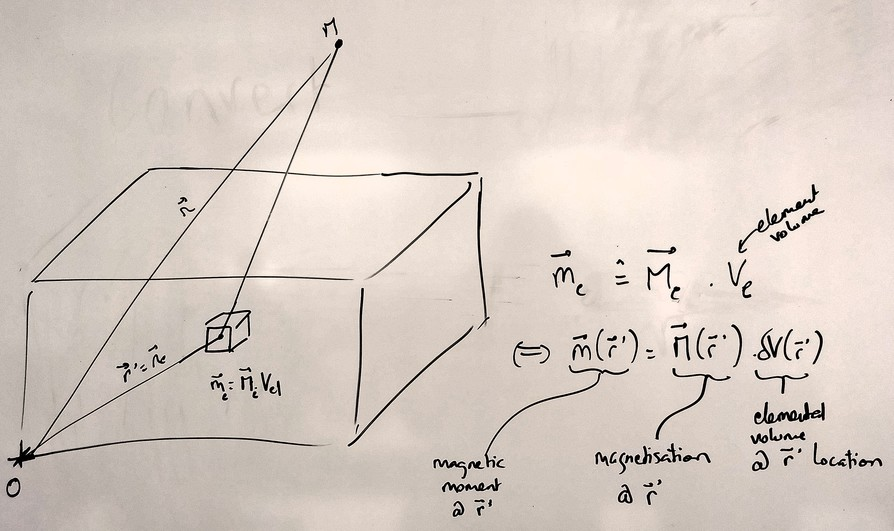
\includegraphics[width=6cm]{python_codes/fieldstone_138/images/01}
\end{center}

The 3D domain $\Omega$ is tesselated with many small volumes (cells).
At any given position $\vec r$, the resulting fields $\vec A$ and $\vec B$
are the sum of the contributions of all cells, assuming each one
can be seen as a dipole $\delta \vec m$.
We then have:
\begin{eqnarray}
\vec A(\vec r) 
&=&  \sum_{i=1,cells} \frac{\mu_0}{4 \pi} \frac{ \delta \vec m_i \times (\vec r- \vec r_{i})}{|\vec r-\vec r_{i}|^3} \\
&=&  \sum_{i=1,cells} \frac{\mu_0}{4 \pi} \frac{ \vec M_i \times (\vec r- \vec r_{i})}{|\vec r-\vec r_{i}|^3} \delta V_i 
\end{eqnarray}
And then, when the number of cells becomes infinitely large, we obtain:
\begin{eqnarray}
\vec A(\vec r) 
&=&  \int_\Omega \frac{\mu_0}{4 \pi} \frac{ \vec M(\vec {r'}) \times (\vec r- \vec {r'})}{|\vec r-\vec{r'}|^3} d\vec{r'} 
\end{eqnarray}
Likewise, the magnetic field is given by 
\begin{eqnarray}
\vec B (\vec r) 
&=& \sum_{i=1,cells} \frac{\mu_0}{4\pi} 
\left[  \frac{3 (\vec r-\vec r_i) (\delta \vec m_i \cdot (\vec r-\vec r_i))}{|\vec r -\vec{r}_i|^5} - \frac{\delta \vec m_i}{|\vec r -\vec{r}_i|^3}  \right] \\
&=& \sum_{i=1,cells} \frac{\mu_0}{4\pi} 
\left[  \frac{3 (\vec r-\vec r_i) (\vec M_i \cdot (\vec r-\vec r_i))}{|\vec r -\vec{r}_i|^5} - \frac{\vec M_i}{|\vec r -\vec{r}_i|^3}  \right] \delta V_i \\
&\dots& \nonumber\\
&=& \int_\Omega \frac{\mu_0}{4\pi} 
\left[ \frac{3 (\vec r-\vec {r'}) (\vec M(\vec {r'}) \cdot (\vec r-\vec{r'}))}{|\vec r -\vec{r'}|^5} - \frac{\vec M(\vec{r'})}{|\vec r -\vec{r'}|^3} \right] d\vec{r'} 
\end{eqnarray}






------------------------------------------------------------------------------
FROM grape function comment latex
This function receives as argument the coordinates {\tt x,y,z} of a point and 
returns the magnetic vector potential ${\bm A}$ and the magnetic field ${\bm B}$
defined by the equations
\begin{eqnarray}
{\bm B}({\bm r}) &=& \frac{\mu_0}{4\pi} \int\int\int \frac{1}{|{\bm r}-{\bm r}'|^3}
\left[
\frac{3}{|{\bm r}-{\bm r}'|^2} [{\bm M}({\bm r}')\cdot({\bm r}-{\bm r}')]({\bm r}-{\bm r}') - {\bm M}({\bm r}')
\right]
d^3{\bm r}' \\
{\bm A}({\bm r}) &=& 
\frac{\mu_0}{4\pi} \int\int\int \frac{{\bm M}({\bm r}') \times ({\bm r}-{\bm r}')}{|{\bm r}-{\bm r}'|^3}
d^3{\bm r}'
\end{eqnarray}
In the SI system, the units of A are $V.s.m^{-1}$ 
and are the same as that of momentum per unit charge.

We can also compute the magnetic scalar potential $\psi$ as follows:
\[
\Psi (\vec r)= \frac{1}{4\pi} \int\int\int \frac{{\vec M}({\vec r}') \cdot ({\vec r}-{\vec r}')}{|{\vec r}-{\vec r}'|^3} 
d^3{\vec r}'
\]
and the magnetic field vector $\vec H$:
\[
\vec H = -\vec\nabla \psi = 
- \int\int\int 
\left[
 M_x({\vec r}') \underbrace{\vec\nabla \frac{ (x-x')}{|{\vec r}-{\vec r}'|^3}}_{\vec\Theta_x} +   
 M_y({\vec r}') \underbrace{\vec\nabla \frac{ (y-y')}{|{\vec r}-{\vec r}'|^3}}_{\vec\Theta_y} +   
 M_z({\vec r}') \underbrace{\vec\nabla \frac{ (z-z')}{|{\vec r}-{\vec r}'|^3}}_{\vec\Theta_z}    
\right] 
d^3{\vec r}'
\]
\begin{eqnarray}
\vec\Theta_x 
&=& \vec\nabla \frac{ (x-x')}{ [(x-x')^2+(y-y')^2+(z-z')^2]^{3/2}   } \\
&=&
\frac{1}{|{\vec r}-{\vec r}'|^6}
\left(\begin{array}{c}
1 \cdot |{\vec r}-{\vec r}'|^3 - (x-x') \cdot 3 (x-x') |{\vec r}-{\vec r}'| \\ \\
0 \cdot |{\vec r}-{\vec r}'|^3 - (x-x') \cdot 3 (y-y') |{\vec r}-{\vec r}'| \\ \\
0 \cdot |{\vec r}-{\vec r}'|^3 - (x-x') \cdot 3 (z-z') |{\vec r}-{\vec r}'| 
\end{array}\right) \\
&=& 
\frac{1}{|{\vec r}-{\vec r}'|^5}
\left(\begin{array}{c}
|{\vec r}-{\vec r}'|^2 - 3(x-x') (x-x')  \\ \\
- 3(x-x')(y-y')  \\ \\
- 3(x-x')(z-z')  
\end{array}\right) \\ 
\vec\Theta_y 
&=& \vec\nabla \frac{ (y-y')}{ [(x-x')^2+(y-y')^2+(z-z')^2]^{3/2}   } \\
&=& 
\frac{1}{|{\vec r}-{\vec r}'|^5}
\left(\begin{array}{c}
- 3(y-y') (x-x')  \\ \\
|{\vec r}-{\vec r}'|^2 - 3(y-y')(y-y')  \\ \\
- 3(y-y')(z-z')  
\end{array}\right) \\ 
\vec\Theta_z 
&=& \vec\nabla \frac{ (z-z')}{ [(x-x')^2+(y-y')^2+(z-z')^2]^{3/2}   } \\
&=& 
\frac{1}{|{\vec r}-{\vec r}'|^5}
\left(\begin{array}{c}
- 3(z-z') (x-x')  \\ \\
- 3(z-z')(y-y')  \\ \\
|{\vec r}-{\vec r}'|^2 - 3(z-z')(z-z')  
\end{array}\right) \\ 
\end{eqnarray}





TODO/TOCHECK:

minus sign: resulting B from vol and surface intergation are opposite signs?

nqdim ? 

atan2? f77 python 

add dtype to arrrays

compute field above vertical face!

explain difference btw m and M (dipole moment vs magnetisation)


%%%%%%%%%%%%%%%%%%%%%%%%%%%%%%%%%%%%%%%%%%%%%%%%%%%%%%%%%%%%%%%%%%%%%%%%%%%%%%
\subsection*{Benchmark 1 - magnetic field above a spherical anomaly/dipole}

The domain is $2\times 2\times 2~\si{\meter}$. No background magnetisation. Single spherical inclusion 
of radius \SI{1}{\meter} in the middle of the domain with magnetisation ${\bm M}=(0,1,0)$. 
Note that the computational domain is such that its top surface is at $z=0$.

If one now computes the magnetic field on a vertical line centered on the sphere, one 
should recover the single dipole value at very large distances ($z>>L_z$). 

We start from the vector potential of a single dipole (Eq. 5.83 of \cite{griffiths}) 
\[
{\bm A}_{dip}({\bm r}) = \frac{\mu_0}{4\pi} \frac{{\bm m}\times {\bm r}}{r^3}.
\]
Very far away from the sphere, one can see the sphere as a single dipole of volume $V=4\pi R^3/\pi$
and $r$ is the distance between the measurement point and the center of the sphere, i.e. $r=z-z_c$:
\[
{\bm A}_{dip}({\bm r}) = \frac{\mu_0}{4\pi} \frac{{\bm M} V\times {\bm r}}{(z-z_c)^3}
\]
Also, ${\bm M}=(0,1,0)$ and ${\bm r}=(x-x_c,y-y_c,z-z_c)=(0,0,z-z_c)$ so that ${\bm M}\times {\bm r}=M (z-z_c) {\bm e}_x$.
Finally:
\[
A_x(z)=\frac{\mu_0}{4\pi} \frac{MV}{(z-z_c)^2}  \quad\quad
A_y=0 \quad\quad
A_z=0
\]
%\begin{center}
%\includegraphics[width=12cm]{images/benchmark_magfield_above_dipole/Ax.pdf}
%\end{center}


Turning to the magnetic field of a single dipole:
\[
{\bm B}_{dip}({\bm r}) = \frac{\mu_0}{4\pi} \frac{1}{r^3} \left[ \frac{3}{r^2} ({\bm m} \cdot {\bm r}) {\bm r} - {\bm m}\right]
\]

\[
{\bm B}_{dip}({\bm r}) = \frac{\mu_0 V}{4\pi} \frac{1}{r^3} \left[ \frac{3}{r^2} ({\bm M} \cdot {\bm r}) {\bm r} - {\bm M}\right]
\]
We have ${\bm M} \cdot {\bm r}=0$ so
\[
{\bm B}_{dip}({\bm r}) = -\frac{\mu_0 V}{4\pi} \frac{M}{r^3}   {\bm e}_y
\]
%\begin{center}
%\includegraphics[width=12cm]{images/benchmark_magfield_above_dipole/By.pdf}
%\end{center}






%%%%%%%%%%%%%%%%%%%%%%%%%%%%%%%%%%%%%%%%%%%%%%%%%%%%%%%%%%%%%%%%%%%%%%%%%%%%%%
\subsection*{Benchmark 2}



%%%%%%%%%%%%%%%%%%%%%%%%%%%%%%%%%%%%%%%%%%%%%%%%%%%%%%%%%%%%%%%%%%%%%%%%%%%%%%
\subsection*{Benchmark 3}



